% Made by: KorG
% vim: ft=tex cc=79 ts=3 sw=3 et
\documentclass[hyperref={unicode=true}]{beamer}
\usepackage[T2A]{fontenc}       % fonts
\usepackage[utf8]{inputenc}     % UTF-8
\usepackage[english,russian]{babel}     % russian
\usepackage{cmap}               % russian search in pdf
\usepackage{pscyr}		        % PSCyr
\usepackage{float}		        % essential for [H]
\usepackage{indentfirst}        % first string indention
\usepackage{graphicx}           % graphics
\usepackage{ltxtable}           % tables
\usepackage{amsmath}            % math
\usepackage{nccmath}            % math
\usepackage{amsfonts}           % math fonts
\usepackage{amssymb}            % math symb
\usepackage{color}
\usepackage{xcolor}
\definecolor{light-gray}{gray}{0.9}
\usepackage{multirow}
\usepackage{tabularx}
\usepackage{placeins}
\usepackage{totcount}
\usepackage{soul}               % \so{} & \ul{} - source and underline
\usepackage{soulutf8}           % UTF-8 for soul
\usepackage{verbatim}           % \verb{} and verbatim environment
\usepackage{listings}           % source code `bl
\usepackage{totcount}
\usepackage{pbox}
\usepackage{rotating}
\lstset{
   escapeinside={\#@}{@},
        extendedchars=\true,
        numbers=none,
        inputencoding=utf8,
        keepspaces=true,
        basicstyle=\large\ttfamily,
        backgroundcolor=\color{light-gray},
        tabsize=3,
        breaklines=true,
        postbreak=\raisebox{0ex}[0ex][0ex]{\ensuremath{
           \color{red}\hookrightarrow\space}
        }
     }

\usebackgroundtemplate{
   \begin{picture}(0,260)
      \minipage{0.9\textwidth}
      
\includegraphics[width=0.6\textwidth]{ifmo.jpg} %TODO check file path
      \endminipage
      \hfill \hspace*{60px}
      \ifnum\value{framenumber}>1 \Large \insertpagenumber \fi
   \end{picture}
}

\setbeamertemplate{navigation symbols}{}

\title{\LARGE Материалы к лекциям \\ по разработке скриптов, \\
   интерпретаторам \\ семейства sh и perl \vspace{2em}}
\author{Жмылёв Сергей Александрович \vspace{-1em}}
\date{Осень 2018}

\begin{document} \Large

\begin{frame} \titlepage \end{frame}

\regtotcounter{section}
\setbeamertemplate{section in toc}{\inserttocsection}
\setbeamercolor{section in toc}{fg=black}
\begin{frame}[allowframebreaks]{Структура курса}
\fontsize{1em}{-1em}\selectfont
\vspace{1em} \tableofcontents[sections=1-8] \vspace{2em}
\ifnum\totvalue{section}>8 \framebreak
\vspace{1em} \tableofcontents[sections=9-16]  \vspace{2em} \fi
\ifnum\totvalue{section}>16 \framebreak
\vspace{1em} \tableofcontents[sections=17-24] \vspace{2em} \fi
\ifnum\totvalue{section}>24 \framebreak
\vspace{1em} \tableofcontents[sections=25-32] \vspace{2em} \fi
\ifnum\totvalue{section}>32 \framebreak
\vspace{1em} \tableofcontents[sections=33-40] \vspace{2em} \fi
\ifnum\totvalue{section}>40 \framebreak
\vspace{1em} \tableofcontents[sections=41-48] \vspace{2em} \fi
\ifnum\totvalue{section}>48 \framebreak
\vspace{1em} \tableofcontents[sections=49-56] \vspace{2em} \fi
\ifnum\totvalue{section}>56 \framebreak
\vspace{1em} \tableofcontents[sections=57-64] \vspace{2em} \fi
\ifnum\totvalue{section}>64 \framebreak
\vspace{1em} \tableofcontents[sections=65-72] \vspace{2em} \fi
\ifnum\totvalue{section}>72 \framebreak
\vspace{1em} \tableofcontents[sections=73-80] \vspace{2em} \fi
\ifnum\totvalue{section}>80 \framebreak
\vspace{1em} \tableofcontents[sections=81-88] \vspace{2em} \fi
\ifnum\totvalue{section}>88 \framebreak
\vspace{1em} \tableofcontents[sections=89-96] \vspace{2em} \fi
\ifnum\totvalue{section}>96 \framebreak
\vspace{1em} \tableofcontents[sections=97-104] \vspace{2em} \fi
\end{frame}

\newcommand{\iframe}[1]{
   \section{#1}\begin{frame}[fragile]{#1}\par\vspace{-1em}
}
\newcommand{\pframe}[1]{
   \begin{frame}[fragile]{#1}\par\vspace{-1em}
}

%%%%%%%%%%%%%%%%%%%%%%%%%%%%%%%%%%%%%%%%%%%%%%%%%%%%%%%%%%%%%%%%%%%%%%%%%%%%%%%
% vim: ft=tex cc=79 ts=3 sw=3 et
% 
% iframe = master frame; pframe = slave frame
\pframe{Организационные вопросы}

Организационный объём курса:
\begin{itemize}
\item 3+ лабораторных по shell
\item 3+ лабораторных по C
\item 2+ рубежных контрольных
\item 1+ письменный зачет
\item ?+ курсовых работ
\end{itemize}

\vspace{0.5cm}
Посещаемость, электронный журнал, баллы, пересдачи, зачетки, отзывы, вопросы.

\end{frame}
 % организационные вопросы
% vim: ft=tex cc=79 ts=3 sw=3 et
% 
\pframe{}

The best teachers are those who show you where to look,
but don't tell you what to see.

\vspace{1cm} \hfill \raggedleft Alexandra K.Trenfor
\end{frame}

\pframe{Полезные ссылки}

\url{https://man.freebsd.org/sh/}

\url{https://perldoc.perl.org/perl.html} \vspace{1em}

Материалы по курсу:

\url{https://se.ifmo.ru/~korg/} \vspace{1em}

Группа ВКонтакте (объявления, вопросы):

\url{https://vk.com/korglings}

\begin{lstlisting}
$ man lcheck
\end{lstlisting}

\end{frame}
 % полезные ссылки
% vim: ft=tex cc=79 ts=3 sw=3 et
% 
% iframe = master frame; pframe = slave frame
\iframe{Взаимодействие с системой}

\begin{columns}
\begin{column}{0.5\textwidth}
\centering
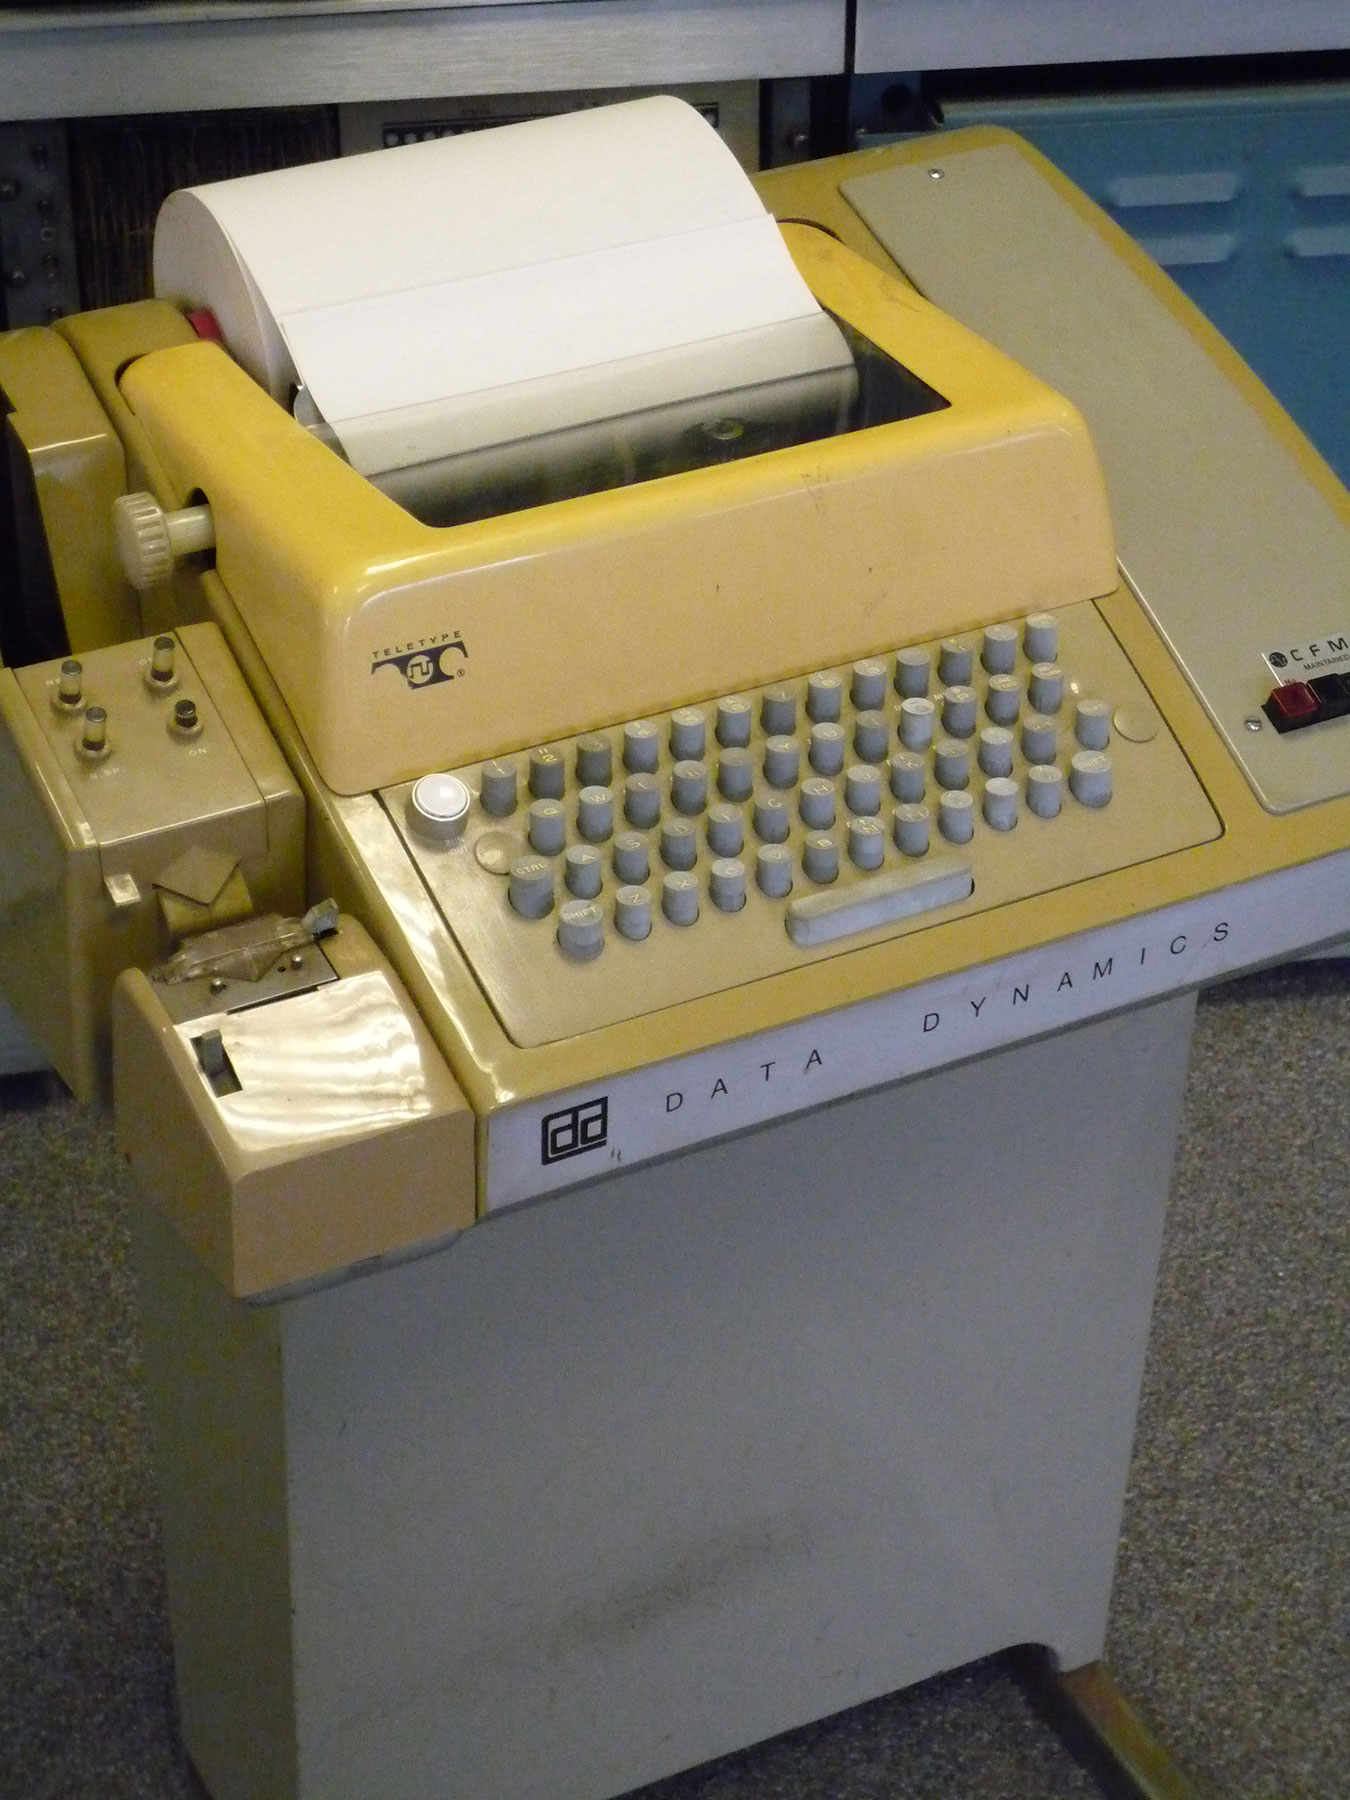
\includegraphics[height=0.8\textheight]{img/teletype.jpg}
\end{column}
\begin{column}{0.5\textwidth}
\hspace{-0.5cm}
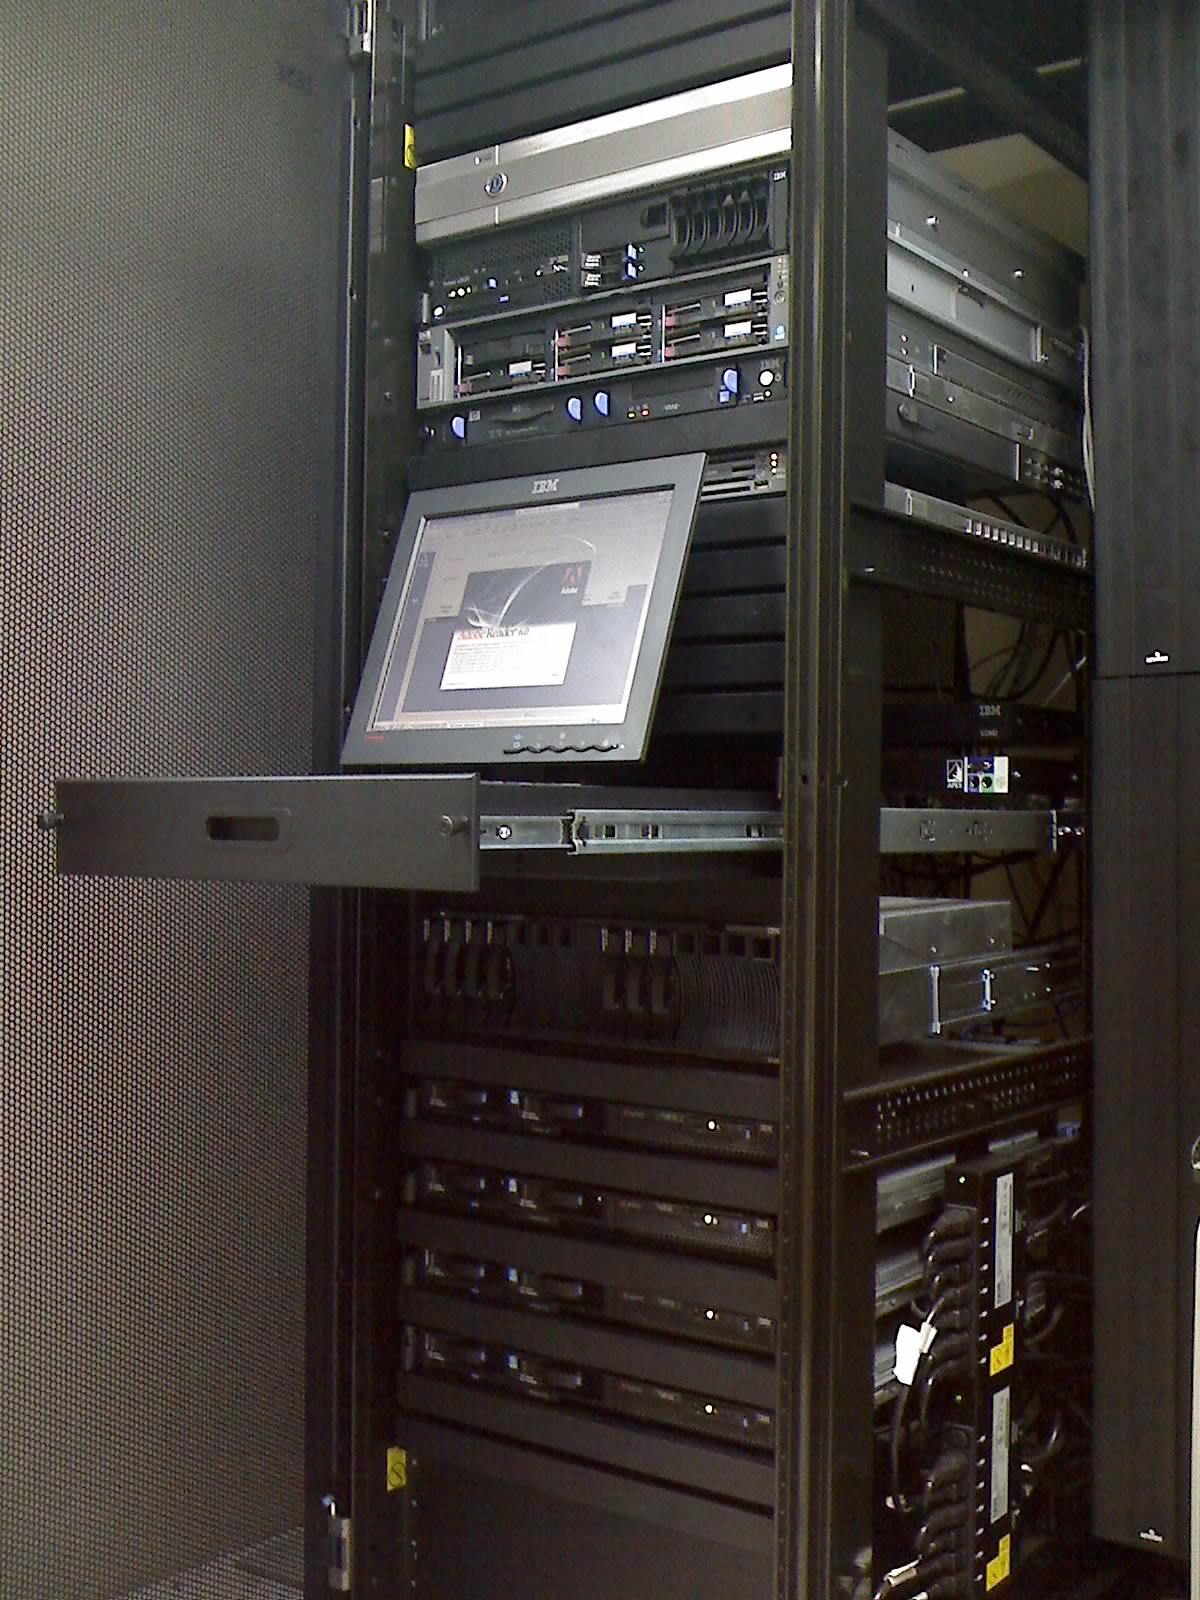
\includegraphics[height=0.8\textheight]{img/console.jpg}
\end{column}
\end{columns}

\end{frame}
 % взаимодействие с системой
% vim: ft=tex cc=79 ts=3 sw=3 et
% 
% iframe = master frame; pframe = slave frame
\iframe{Философия UNIX}

Write programs that do one thing and do it well.
Write programs to work together.
Write programs to handle text streams, because that is a universal interface.
\\ \hfill Peter H. Salus.

\pause

Clarity is better than cleverness.
In interface design, always do the least surprising thing.
When a program has nothing surprising to say, it should say nothing.
\\ \hfill Eric S. Raymond.

\vfill

\small
\hspace{-0.2cm}\url{http://catb.org/esr/writings/taoup/html/ch01s06.html}

\end{frame}

\pframe{Принцип KISS}

\centering
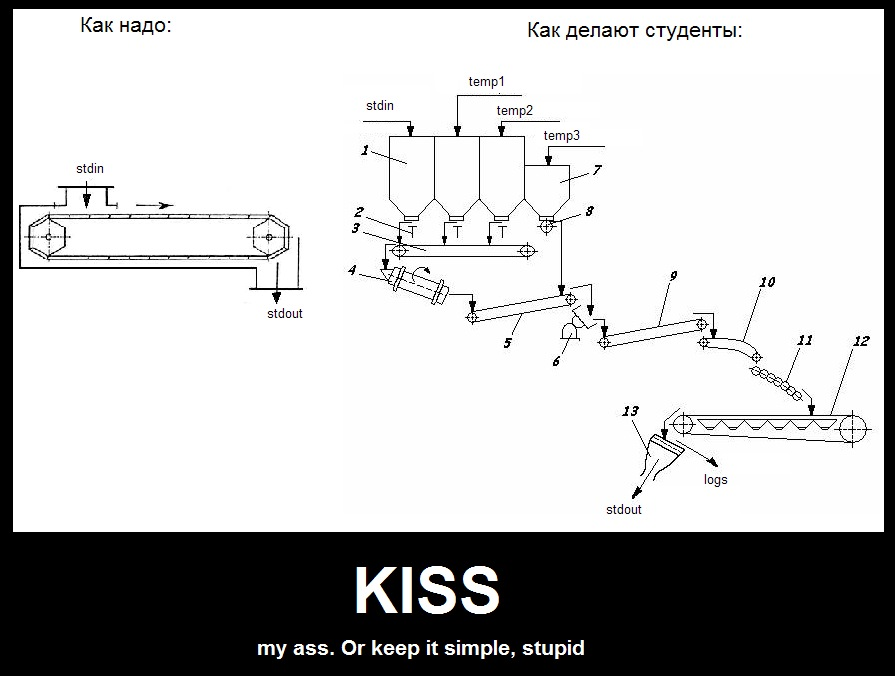
\includegraphics[width=0.9\textwidth]{img/kiss.jpg}

\end{frame}
 % философия UNIX
% vim: ft=tex cc=79 ts=3 sw=3 et
% 
% iframe = master frame; pframe = slave frame
\iframe{Потоки ввода-вывода}

-- это записи из таблицы дескрипторов открытых файлов для \textbf{процесса}.

\begin{table}[H]
\centering
\begin{tabular}{|c|c|c|}
\hline
\textbf{Номер} & \textbf{Файл} & \textbf{Флаги} \\
\hline 0 & файл с паролями & чтение \\ 
\hline 1 & терминал & запись \\
\hline ... & & \\
\hline 255 & & \\
\hline
\end{tabular}
\end{table}

\begin{itemize}
\item 0 -- стандартный поток ввода (stdin)
\item 1 -- стандартный поток вывода (stdout)
\item 2 -- стандартный поток ошибок (stderr)
\end{itemize}

\end{frame}
 % потоки ввода-вывода
% vim: ft=tex cc=79 ts=3 sw=3 et
% 
\iframe{Shell}

-- a software tool designed to:
\begin{enumerate}
   \item read commands from file or terminal
   \item interpret them
   \item organize execution of programs
\end{enumerate}

\vspace{1cm}

login shell -- user property that defines a default command being executed on logon.
\begin{lstlisting}
$ getent passwd korg |cut -d: -f7
/usr/bin/bash
\end{lstlisting}

\end{frame}

\pframe{Shell basic functionality}

\begin{itemize}
\item Command flow control
\\... and their automation.
\item Macro substitutions
\item Command line management (edit, libreadline, ...)
\item History of executed commands
\item Scripts execution
\end{itemize}

\end{frame}
 % командный интерпретатор
% vim: ft=tex cc=79 ts=3 sw=3 et
% 
% iframe = master frame; pframe = slave frame
\iframe{Разновидности интерпретаторов}

\begin{tabular}{|lcc}
\hline
& & \textbf{Скриптовые} \\
& \parbox{4.5cm}{---} & 
\parbox{4.5cm}{\raggedright js, php, python, Tcl \\ perl, ruby} \\
\rotatebox{90}{\hspace{-0.5cm}\textbf{Интерактивные}\hspace{1.5cm}} &
\parbox{4.5cm}{sh, ksh, bash,\\ zsh, jsh,\\ csh, tcsh, ...} &
\parbox{4.5cm}{PowerShell\\  Cisco IOS\\ sqlplus}
\end{tabular}

\end{frame}
 % разновидности интерпретаторов

\iframe{Командный файл (скрипт)}
\end{frame}

\iframe{Комментарии}
\end{frame}

\iframe{Команды: утилиты, функции, ...}
\end{frame}

\iframe{Перечень часто используемых утилит}
\end{frame}

\iframe{Переменные окружения}
\end{frame}

\iframe{Переменные интерпретатора}
\end{frame}

\iframe{Ввод-вывод}
\end{frame}

\iframe{Оператор присваивания}
\end{frame}

\iframe{Типы данных: shell}
\end{frame}

\iframe{Типы данных: perl}
\end{frame}

\iframe{Математические операции}
\end{frame}

\iframe{Группировка операций}
\end{frame}

\iframe{Последовательное выполнение: $\&\&, ||, ...$}
\end{frame}

\iframe{Условные операторы $if, then, elif, else, fi$}
\end{frame}

\iframe{Оператор $case$}
\end{frame}

\iframe{Паттерн-матчинг и глоб-джокеры}
\end{frame}

\iframe{Проверка статуса файлов}
\end{frame}

\iframe{Операторы $test, [, [[, !$}
\end{frame}

\iframe{Операторы цикла $while, for, ...$}
\end{frame}

\iframe{Оператор $select$}
\end{frame}

\iframe{Опции интерпретаторов $set$}
\end{frame}

\iframe{Переменные Prompt String}
\end{frame}

\iframe{Работа с аргументами скрипта $\$@,\$*,shift$}
\end{frame}

\iframe{Функции}
\end{frame}

\iframe{Command Substitution}
\end{frame}

\iframe{Команды $exec, eval$}
\end{frame}

\iframe{Перенаправление ввода-вывода, Here-document}
\end{frame}

\iframe{Parameter Expansion и стандартные значения}
\end{frame}

\iframe{Переменная IFS}
\end{frame}

\iframe{(t)csh: история, где встречается, концептуальные
   и синтаксические отличия}
\end{frame}

% vim: ft=tex cc=79 ts=3 sw=3 et
% 
\pframe{Благодарности}

\begin{itemize}
\item Афанасьев Дмитрий Борисович
\item Горская Александра Андреевна
\item Ховалкина Ксения Николаевна
\item Киреев Валерий Юрьевич
\item и многие другие...
\end{itemize}

\end{frame}
 % благодарности
%%%%%%%%%%%%%%%%%%%%%%%%%%%%%%%%%%%%%%%%%%%%%%%%%%%%%%%%%%%%%%%%%%%%%%%%%%%%%%%
\usebackgroundtemplate{}
\begin{frame}[fragile]
\vspace{3em}
\centering \LARGE Спасибо за внимание

\vspace{4em}
\begin{tabular}{c}
\begin{lstlisting}[basicstyle=\tiny]
# perl '-es!!),-#(-.?{<>-8#=..#<-*}>;*7-86)!;y!#()-?{}!\x20/`-v;<!;s++$_+ee'
\end{lstlisting} 
\end{tabular}
\end{frame}

\end{document}
